
\documentclass[../main.tex]{subfiles}
%!TEX root = ./analysisSystemModelling.tex
\graphicspath {{../}}

\begin{document}
\subsection{Thrusters} \label{thrusterIntro}
The thruster will be balanced so that the servo motor will only use power when actively rotating the thruster. As a result, when the thruster is vectored straight forward, it will not be able to move the shaft assembly due to the inertia of the parts and the minimal resistance in the servo motor. The same effect will be present when the thruster is vectored vertically.\\

Given the high angular velocity and non-negligible inertia of the propeller, the system will be subject to gyroscopic forces if the thruster orientation is changed in flight. To counter the addition of unwanted high forces to the components, power to the thruster will be cut and if need be, applied in the reverse orientation for a specific duration before the thruster is reoriented. This reduction or elimination of angular velocity will effectively render gyroscopic forces negligible or eliminate them all together. \\

Also, the analysis done on the thruster motor did not present considerable results and can be found in Appendix section \ref{vectoringMotor}. The propeller will be well balanced eliminating any detrimental rotating imbalances. The motor mounting bracket will secure the motor using screws, which do not need to be analysed as the stresses applied are negligible compared to the strength of the material.

\subsection{Gondola Forces} \label{gondForces}
In order to complete the analysis on the gondola there are numerous forces and reaction that need to be computed. Reaction forces are solved using the \textit{gondolaForces} code (Section \ref{code:gondolaforce}) in conjunction with \textit{forceSolver} which is explained in Section \ref{forceSolver} (code located in Appendix \ref{code:forceSolver}) and  the \textit{rotate} code (Appendix \ref{code:rotate}).\\

The \textit{gondolaForces} code requires the inputs of all the known forces acting on the gondola and their positions including the drive force of the friction wheel motor, the spring force acting on the friction wheel, the maximum thruster acceleration, the weight of each gondola car, and the linear actuator holding force. The code also requires the pitch angle of the airship ($\phi$), the thruster angle ($\beta$), the angle between the gondola cars($\Theta$) and the position of each bearing arm reaction. All of the angles mentioned above are with reference to the top surface of the rear gondola. The code will output acceleration of the gondola, the maximum force applied on the bearing arms and the holding force if the linear actuator is applied. \\


The coordinate system $x'yz'$ in which all the forces are referenced, is based on the orientation rear gondola (gondola 1) as seen in Figure \ref{fig:bentGondolaSideAllForce}. The code first takes the drive force and the spring force both of which are acting on the friction wheels and rotates them into the coordinated system of the rear gondola based on the 45$^{\circ}$ angle of the torsion hinge. The spring force and drive force acting on the front gondola (gondola 2) are again rotated based on the angle between the gondolas ($\Theta$). Then the code takes the inputed maximum thrust acceleration, rotates it based on the thrust angle ($\beta$) multiplies it by the mass of each gondola car and applies it to the centre of mass of the corresponding gondola car. The mass of each car is then based on the pitch angle ($\phi$) is then also applied to the centre of mass of each gondola car. For the case where the linear actuator is applied that force is included and the holding force in the x-direction is equated to the sum of all other forces acting in that direction up to the maximum capable holding. The maximum capable holding is determined in the linear actuator analysis \ref{linearActuator}. All of the aforementioned forces and angles can be see acting on the gondolas in Figures \ref{fig:bentGondolaSideAllForce} and \ref{fig:bentGondolaTopAllForce}. \\

\begin{figure}[H]
	\centering
	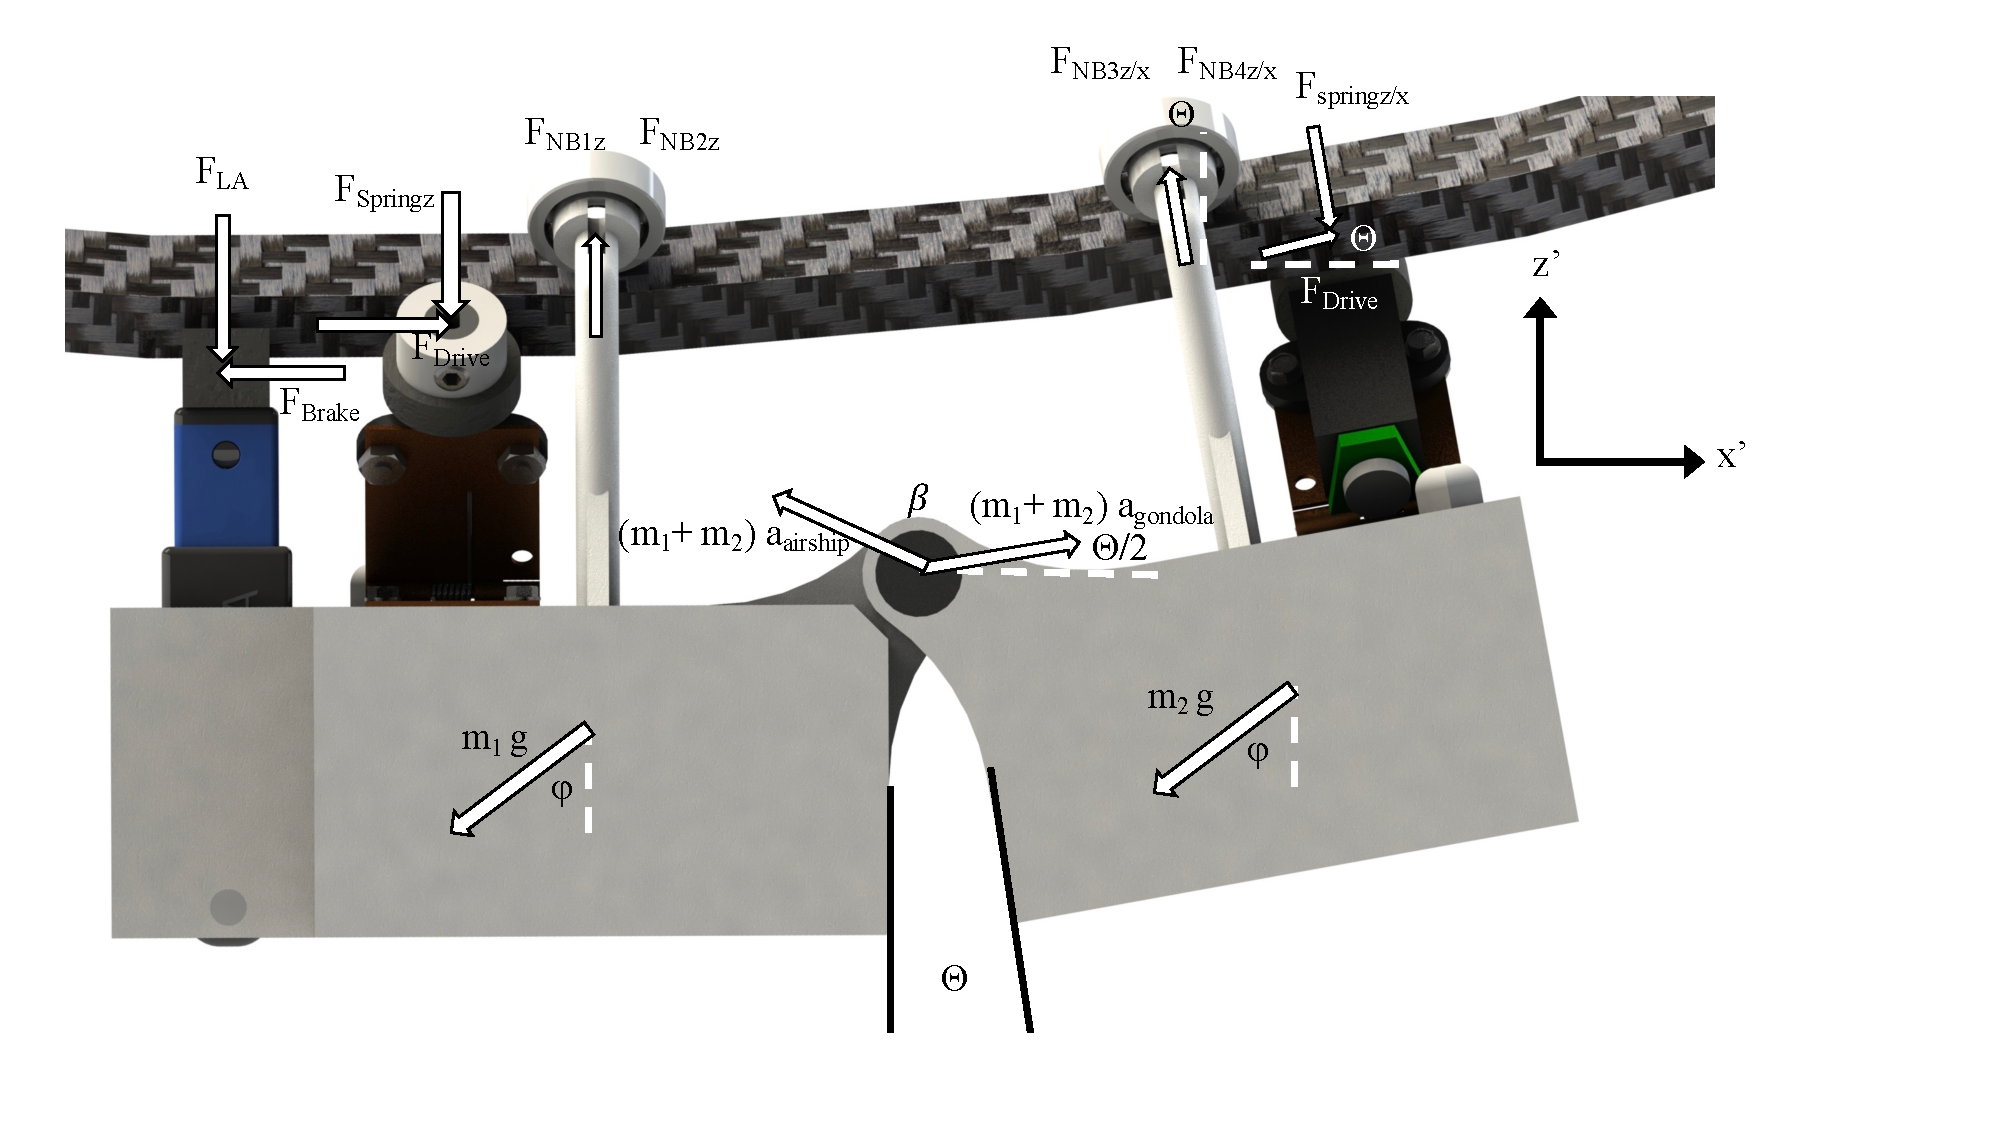
\includegraphics[width=1\linewidth]{img/gondola/bentGondolaSideAllForces.pdf}
	\caption{Side View of Gondola With All Possible Forces and Reactions}
	\label{fig:bentGondolaSideAllForce}
\end{figure}
\begin{figure}[H]
	\centering
	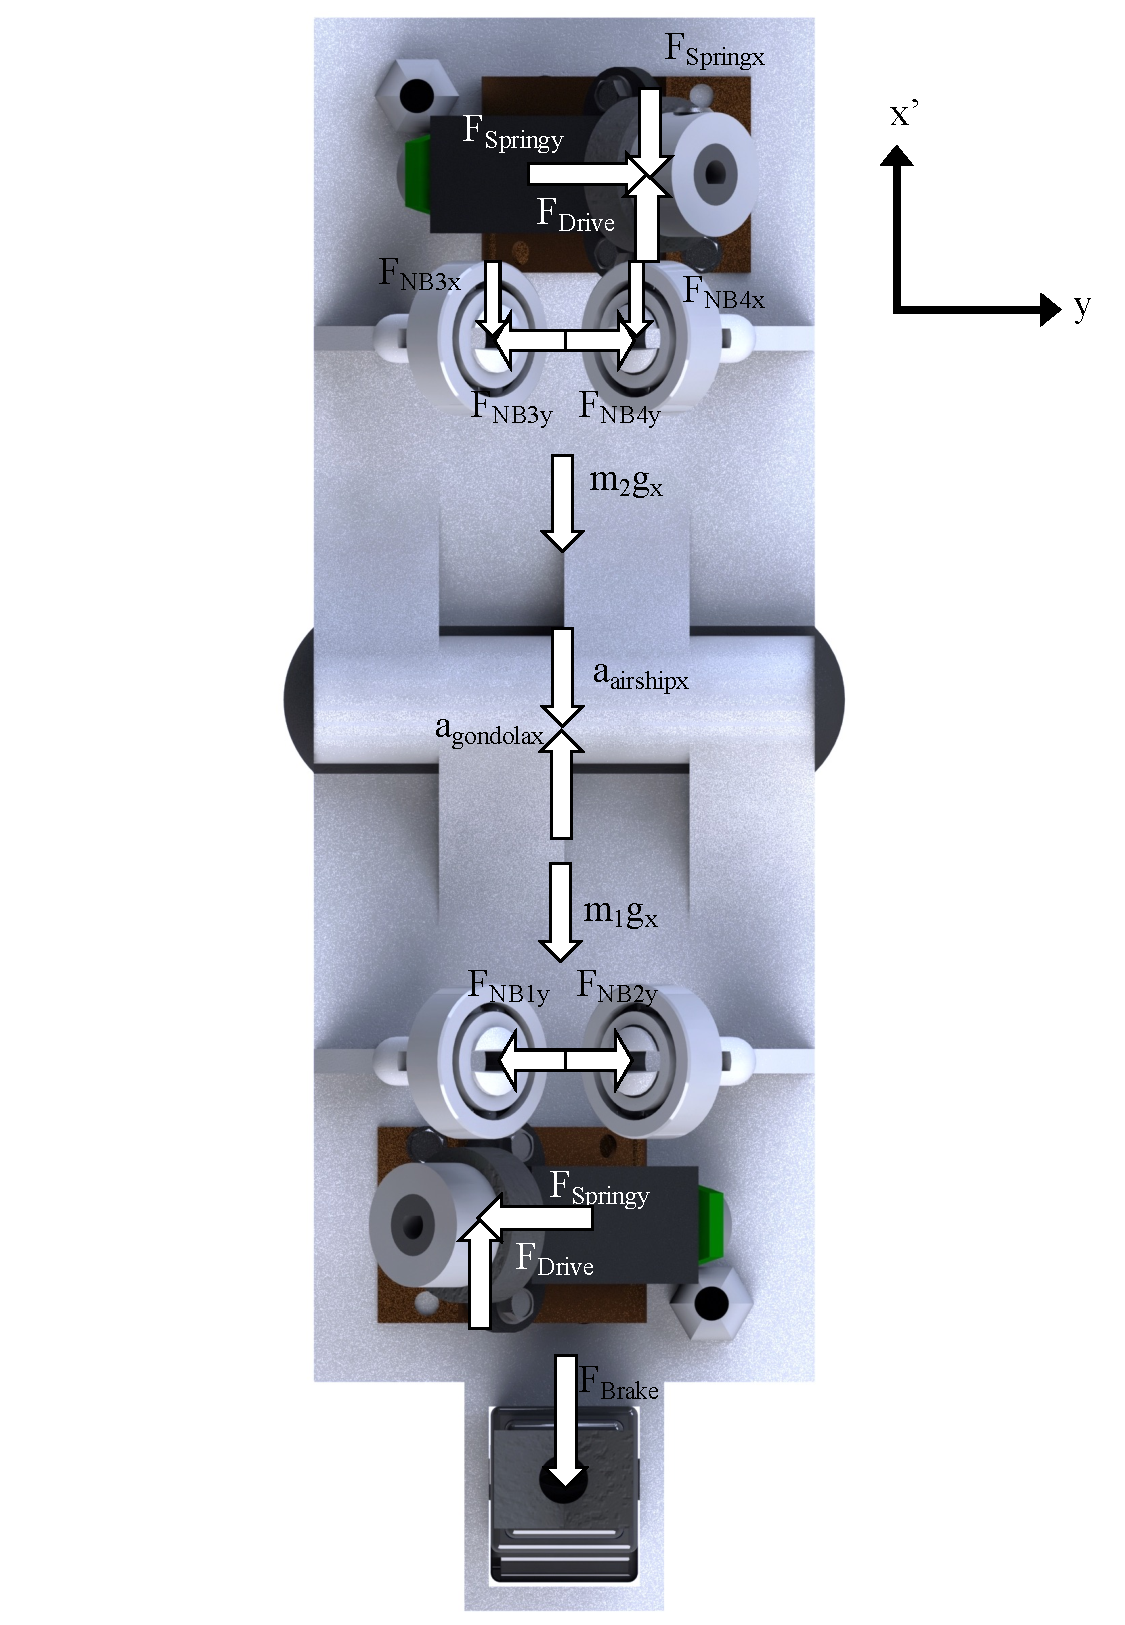
\includegraphics[width=1\textwidth]{img/gondola/bentGondolaTopAllForces.pdf}
	\caption{Top View of Gondola With All Possible Forces and Reactions}
	\label{fig:bentGondolaTopAllForce}
\end{figure}

The sum of forces in $x'y$ and $z'$ in their most general form are presented below with the reactions on the left of the equal sign and the forces on the right.
\begin{multline} \label{Fxgond}
\Sigma F_{x} : (m_{1}+m_{2}) a_{gondola} + F_{NB3_{x}} + F_{NB4_{x}}  =\\ \sin(\phi) (m_{1} + m_2)g + F_{Drive} + \cos (\Theta) F_{Drive} + \cos(\beta) (m_1+m_2) a_{Thrust} + sin(\Theta) F_{Springz} + F_{Brake}
\end{multline}
\begin{flalign} \label{Fygond}
\hspace{12pt}\Sigma F_{y} : -F_{NB1_{y}} + F_{NB2_{y}} - F_{NB3_{y}} + F_{NB4_{y}} =  F_{Springy} - F_{Springy} &&
\end{flalign}
\begin{multline} \label{Fzgond}
\Sigma F_{z} : F_{NB1_{z}} + F_{NB2_{z}} + F_{NB3_{z}} + F_{NB4_{z}} =\\ \cos(\phi) (m_{1} + m_2)g -  cos(\Theta) F_{Springz} - F_{Springz} + \sin(\beta) (m_1+m_2) a_{Thrust}+\sin (\Theta) F_{Drive} + F_{LA}
\end{multline}

The spring forces $F_{Springz}$ and $F_{Springy}$ are acting on the keel at 45\textdegree. They are both the result of the spring torque $T_{Spring}$ shown in equation \ref{eqn:springForce} in the friction wheel slip analysis section \ref{frictionSlip}. Therefore the following equation can be used to define the spring forces. 
\begin{equation}
F_{Springz} = F_{Springy} = \frac{\sqrt{2}}{2} F_{Spring}
\end{equation}
\textit{forceSolver} is used to solve these equations while making some assumptions based on the reactions. All of the $F_{NB}$ the normal forces between the bearings and the keel. since the contact surface is at 45\textdegree between the $xy$ and $xz$ planes, the magnitudes of the forces acting in the y- and z-directions must be equal. 
\begin{align}
\label{eqn:scenario2start}
F_{NB1_{z}} &= - F_{NB1_{y}} \\
F_{NB2_{z}} &= F_{NB2_{y}} 
\end{align}

For the bearings on the front gondola as a result of the angle between gondolas, there will also be a force acting in the x-direction such that:
\begin{align}
F_{NB3_{x}} &= -\tan(\Theta) F_{NB3_{z}}\\ 
F_{NB4_{x}} &= -\tan(\Theta) F_{NB4_{z}}\\
F_{NB3_{y}} &= -\frac{F_{NB3_{z}}}{\cos(\Theta)} \\ F_{NB4_{y}} &= \frac{F_{NB4_{z}}}{\cos(\Theta)} \label{eqn:scenario2end}
\end{align}
The above equations from \ref{eqn:scenario2start} to \ref{eqn:scenario2end} are all encompassed by the switch case, scenario 2, in the \textit{forceSolver} code. 


\subsection{Loading Scenarios} \label{loadingScenarios}
\subsubsection*{Maximum Downward Force (Thrust Force and Gravity Acting Together)}
The scenario shown in Figure \ref{fig:scenario1} would require the greatest drive force from the gondola friction wheel motors. The assumptions made for this scenario are conservative, in that the scenario is unlikely to actually occur but would result in considerably greater forces acting against the gondola motors. The scenario involves the airship pitching straight upwards (pitch angle $\phi$ of 90$^{\circ}$),thrusting straight upwards at full thrust (thrust angle $\beta$ of 0$^{\circ}$) and the gondola is on the straight section of the keel (gondola angle $\Theta$ of 0$^{\circ}$) driving up towards the curved section of the keel.

\begin{figure}[H]
	\centering
	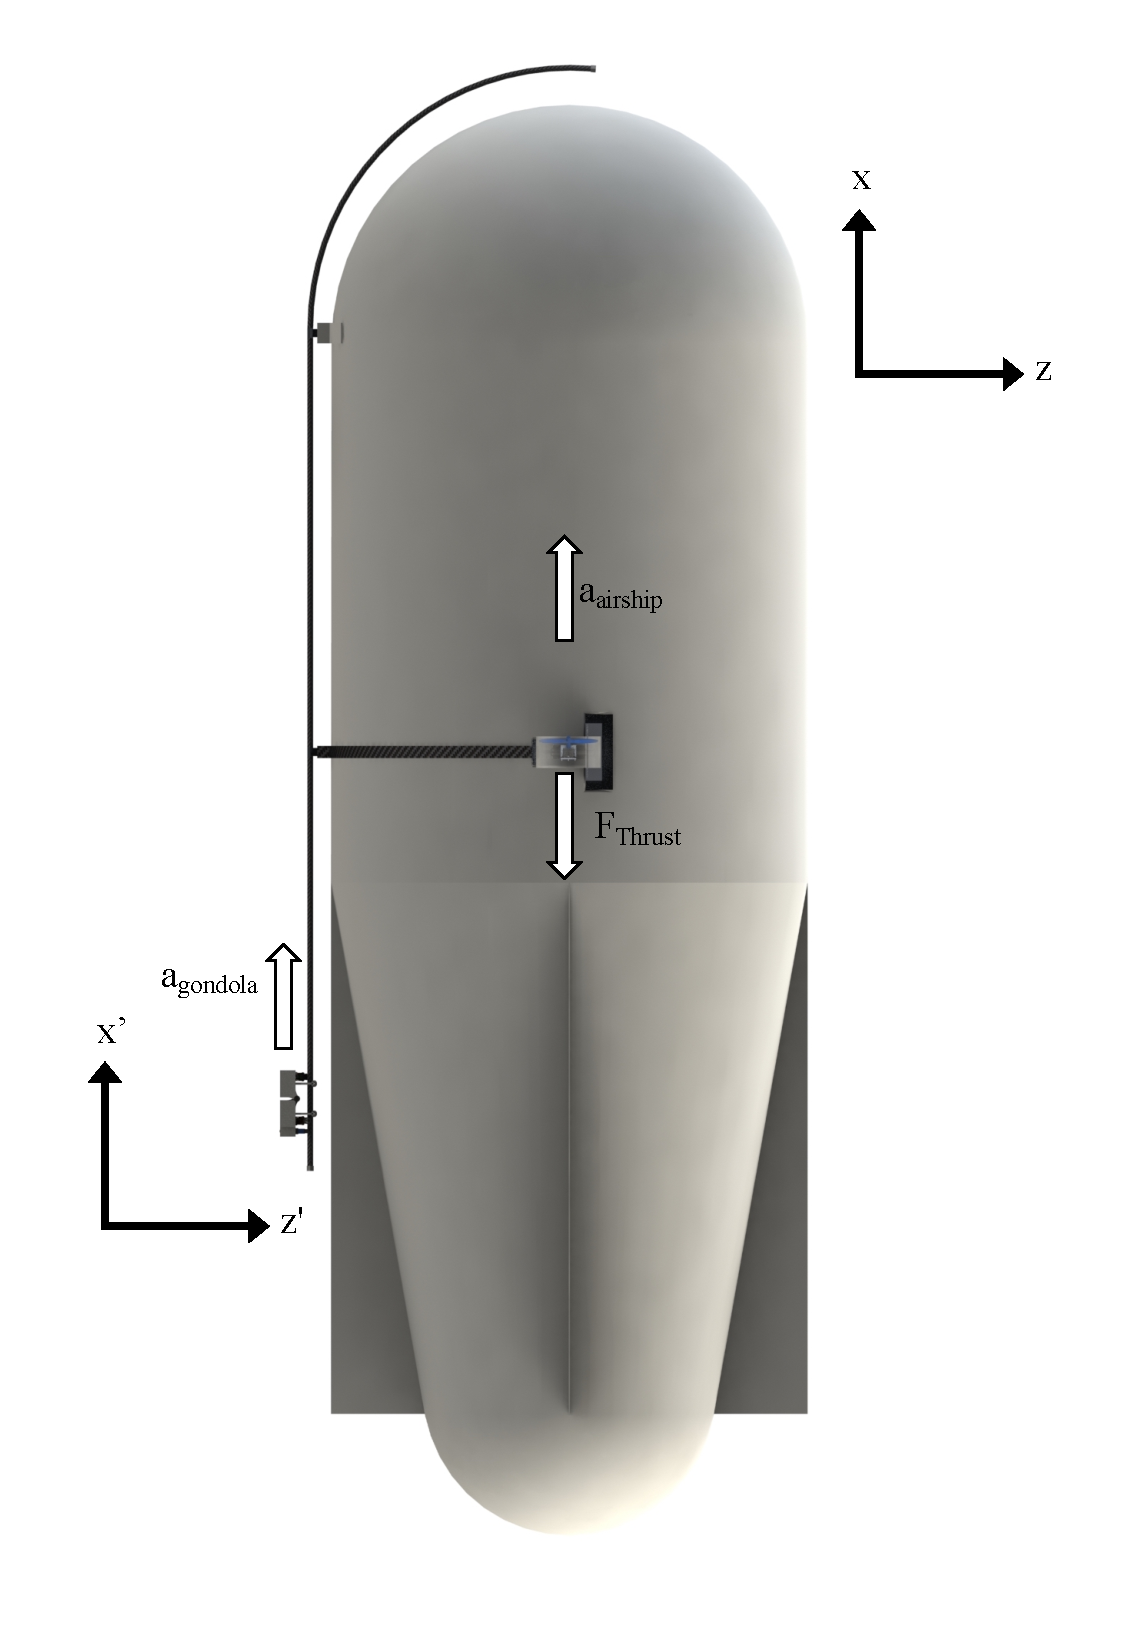
\includegraphics[width=0.5\textwidth]{img/analysis/scenario1.pdf}
	\caption{Side View of Maximum Downward Force Worst-Case Scenario}
	\label{fig:scenario1}
\end{figure}

\subsubsection*{Maximum Gondola Bearing Arm Forces}
The scenario shown in Figure \ref{fig:scenario2} results in the largest forces being applied to the gondola bearing arms. It involves the linear actuator being applied in order to hold the position of the gondola on the straight part of the keel. The airship has a pitch angle of 0$^{\circ}$ and the thrusters is angle is 90$^{\circ}$ straight up. This loading scenario results in the largest force being applied to the bearing arms.

\begin{figure}[H]
	\centering
	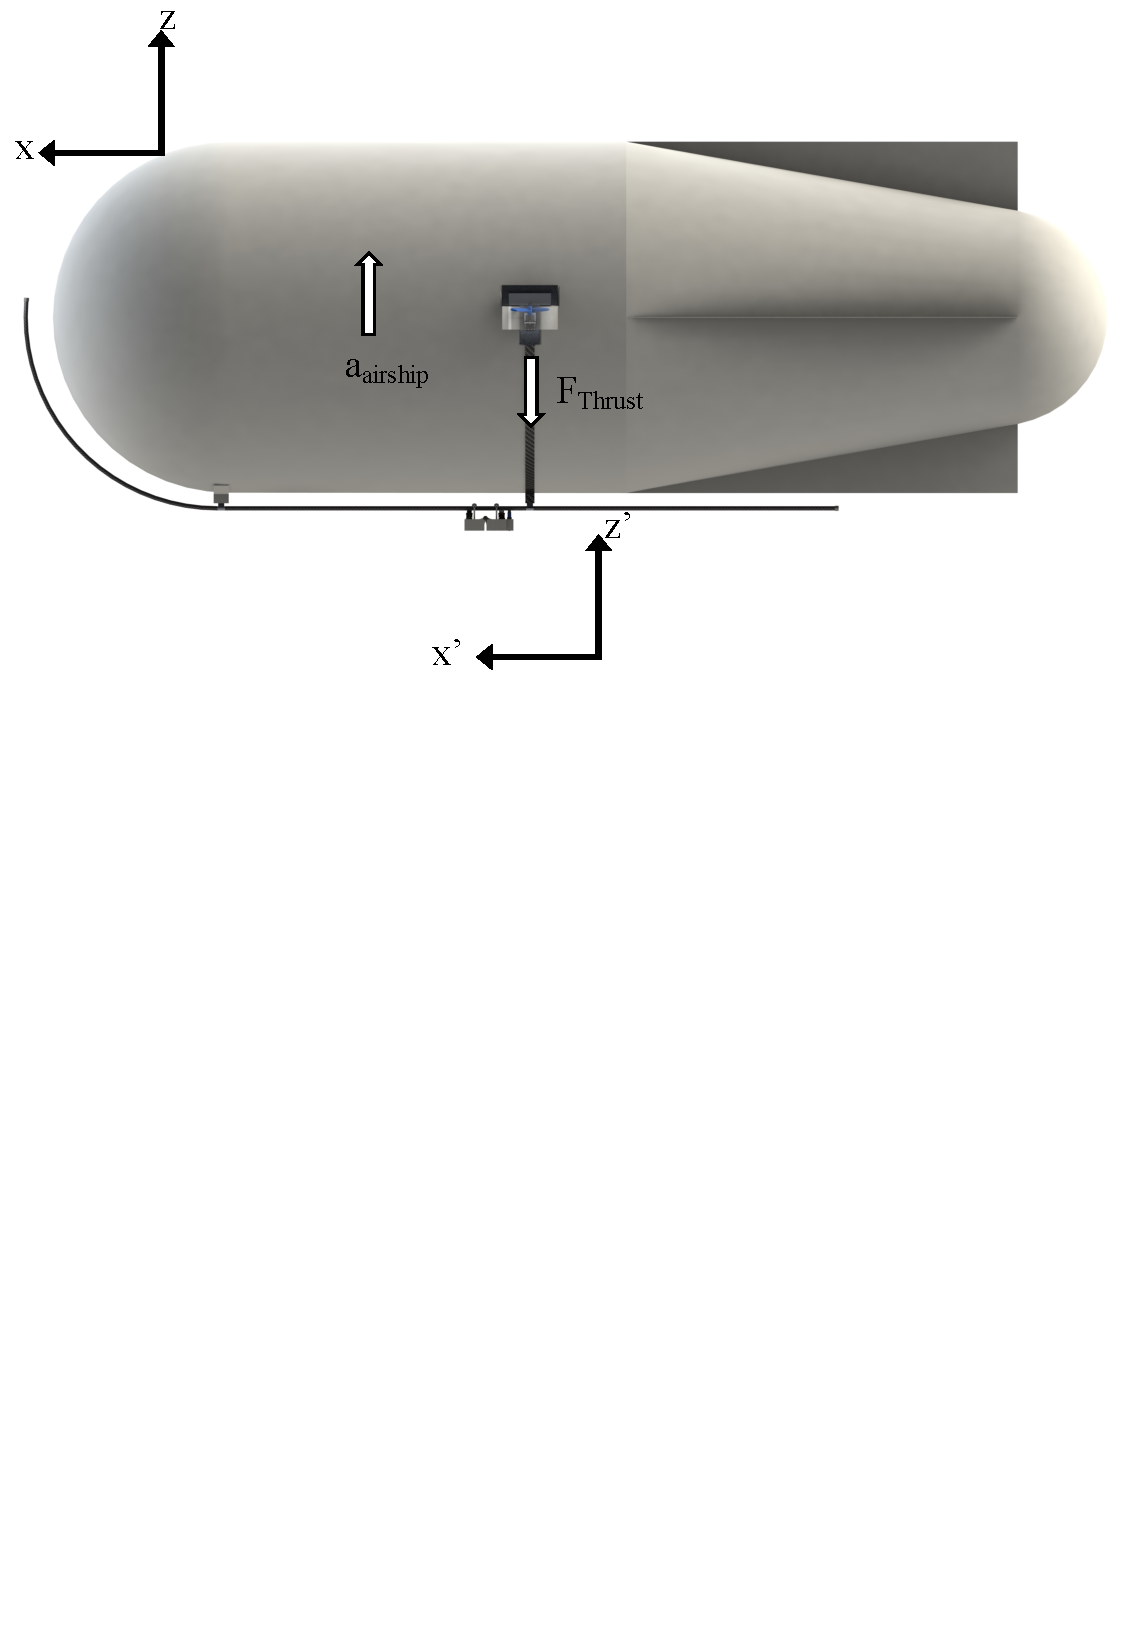
\includegraphics[width=1\textwidth]{img/analysis/scenario2.pdf}
	\caption{Side View of Maximum Gondola Bearing Arm Forces Worst-Case Scenario}
	\label{fig:scenario2}
\end{figure}
\end{document}